
\begin{frame}
    \frametitle{One-Sentence Background}
    In the simplest terms: 
    \begin{center}
        \begin{figure}
            \centering
            \begin{subfigure}[c]{5cm}
                \centering
                \includegraphics<1->[width=3cm]{img/antenna.png}                
            \end{subfigure}
            \begin{subfigure}[c]{2cm}
                \centering
                \uncovergraphics<2->[width=\textwidth]{img/meteor.pdf}
            \end{subfigure}
            \begin{subfigure}[c]{5cm}
                \centering
                \uncovergraphics<3->[width=2cm]{img/wind.pdf}        
            \end{subfigure}            
        \end{figure}
        \onslide<1->{{\textbf{Radar waves}}} \onslide<2->{bounce off \textbf{meteor trails}} \onslide<3->{to learn about the \textbf{wind}}%
        \begin{figure}
            \centering
            \begin{subfigure}[t]{5cm}
                \centering
                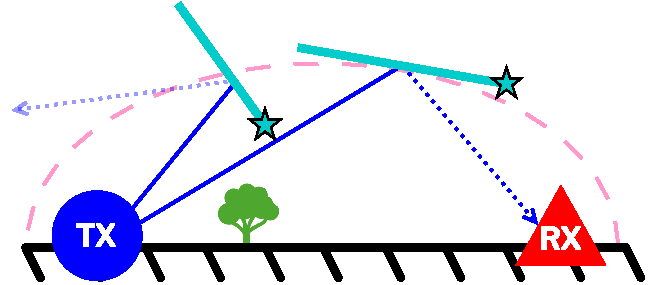
\includegraphics[width=5cm]{img/bistatic_scatter.pdf}
            \end{subfigure}
            \begin{subfigure}[t]{2cm}
                \centering
                \uncovergraphics<2->[width=2cm]{img/mcmurdo_ortho.png}
            \end{subfigure}
            \begin{subfigure}[t]{5cm}
                \centering
                \uncovergraphics<3->[width=5cm]{img/seasonal_trends.pdf}        
            \end{subfigure}            
        \end{figure}
    \end{center}
\end{frame}
